\documentclass[11pt,ngerman]{article}
\usepackage{geometry}
\usepackage[T1]{fontenc}
\usepackage[utf8]{inputenc}
\usepackage{babel}
\usepackage{hyperref}
\usepackage{lmodern}%get scalable font
\usepackage{titling}
\usepackage{relsize}
\usepackage{biblatex}
\usepackage{glossaries}
\usepackage{paralist}
\usepackage[table, dvipsnames]{xcolor}
\usepackage{booktabs}
\usepackage{tabularx}
\usepackage{float}
\restylefloat{table}
\usepackage{setspace}
\usepackage{multicol}
\usepackage{graphicx}
\usepackage[space]{grffile}
\usepackage[most]{tcolorbox}
\usepackage{enumitem}
\usepackage{textcomp}
\usepackage{listings}

% Link colors
\hypersetup{
    colorlinks,
    linkcolor={blue},
    citecolor={red},
    urlcolor={blue}
}

\geometry{a4paper, top=25mm, left=25mm, right=25mm, bottom=20mm,
    headsep=10mm, footskip=12mm}

% inline code macro
\definecolor{lightgray}{gray}{0.9}
\lstset{
    showstringspaces=false,
    basicstyle=\ttfamily,
    keywordstyle=\color{blue},
    commentstyle=\color[grey]{0.6},
    stringstyle=\color[RGB]{255,150,75}
}
\newcommand{\inlinecode}[2]{\colorbox{lightgray}{\lstinline[language=#1]$#2$}}

% Glossary
% Das Glossar definiert alle wichtigen Begriffe zur Sicherstellung einer einheitlichen Terminologie.
% Es sollen keine allgemeinen Begriffe erklärt werden, die den Adressaten bekannt sind (z. B. Java, CPU etc.).

\pretitle{\begin{center}\linespread{1.5}\huge}
    \posttitle{\par\end{center}\vspace{0.5em}}

% double quotes macro
% usage: \quotes{arg1}  => in text: "arg1"
\newcommand{\quotes}[1]{``#1''}

% Image title page
%\pretitle{
%    \begin{center}
%    \begin{figure}[H]
%        \centering
%        \makebox[\textwidth][c]{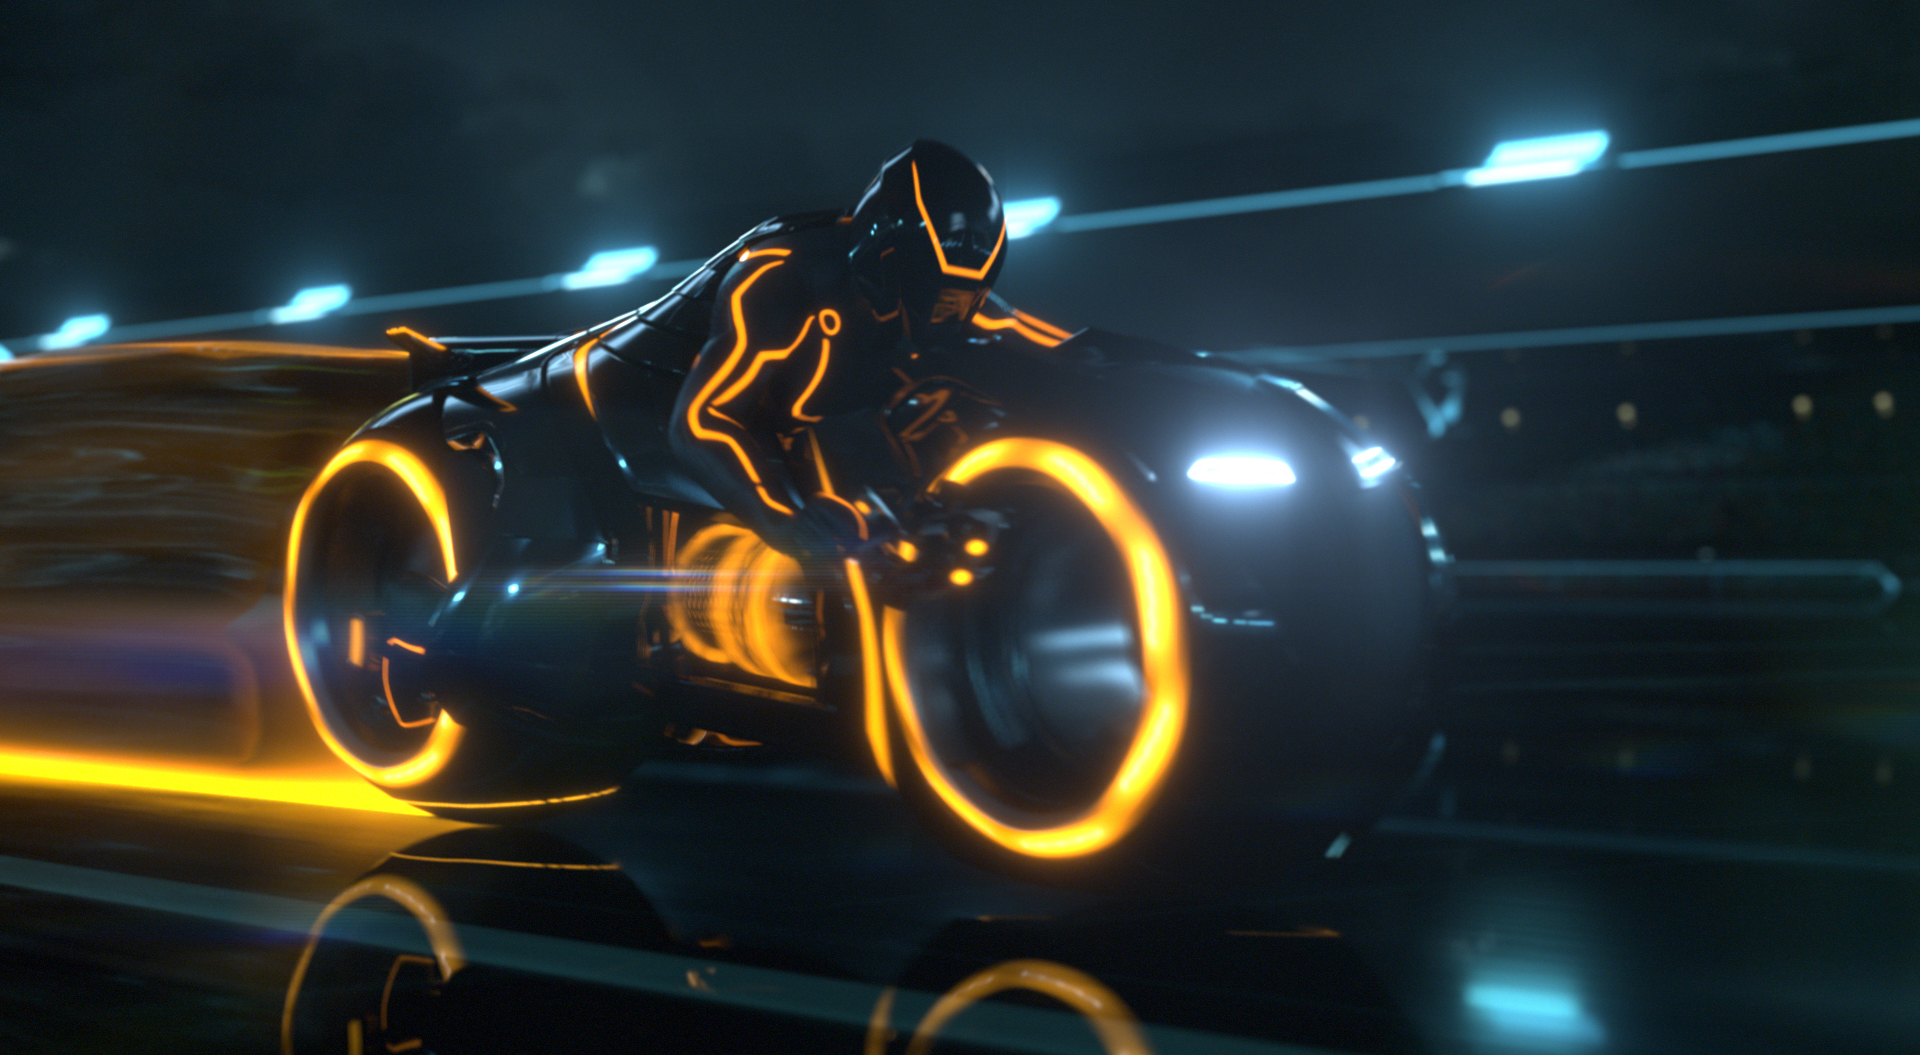
\includegraphics[width=1.2\textwidth]{figures/Tron-Legacy_Bike.jpg}}
%    \end{figure}
%}

\begin{document}
    \title{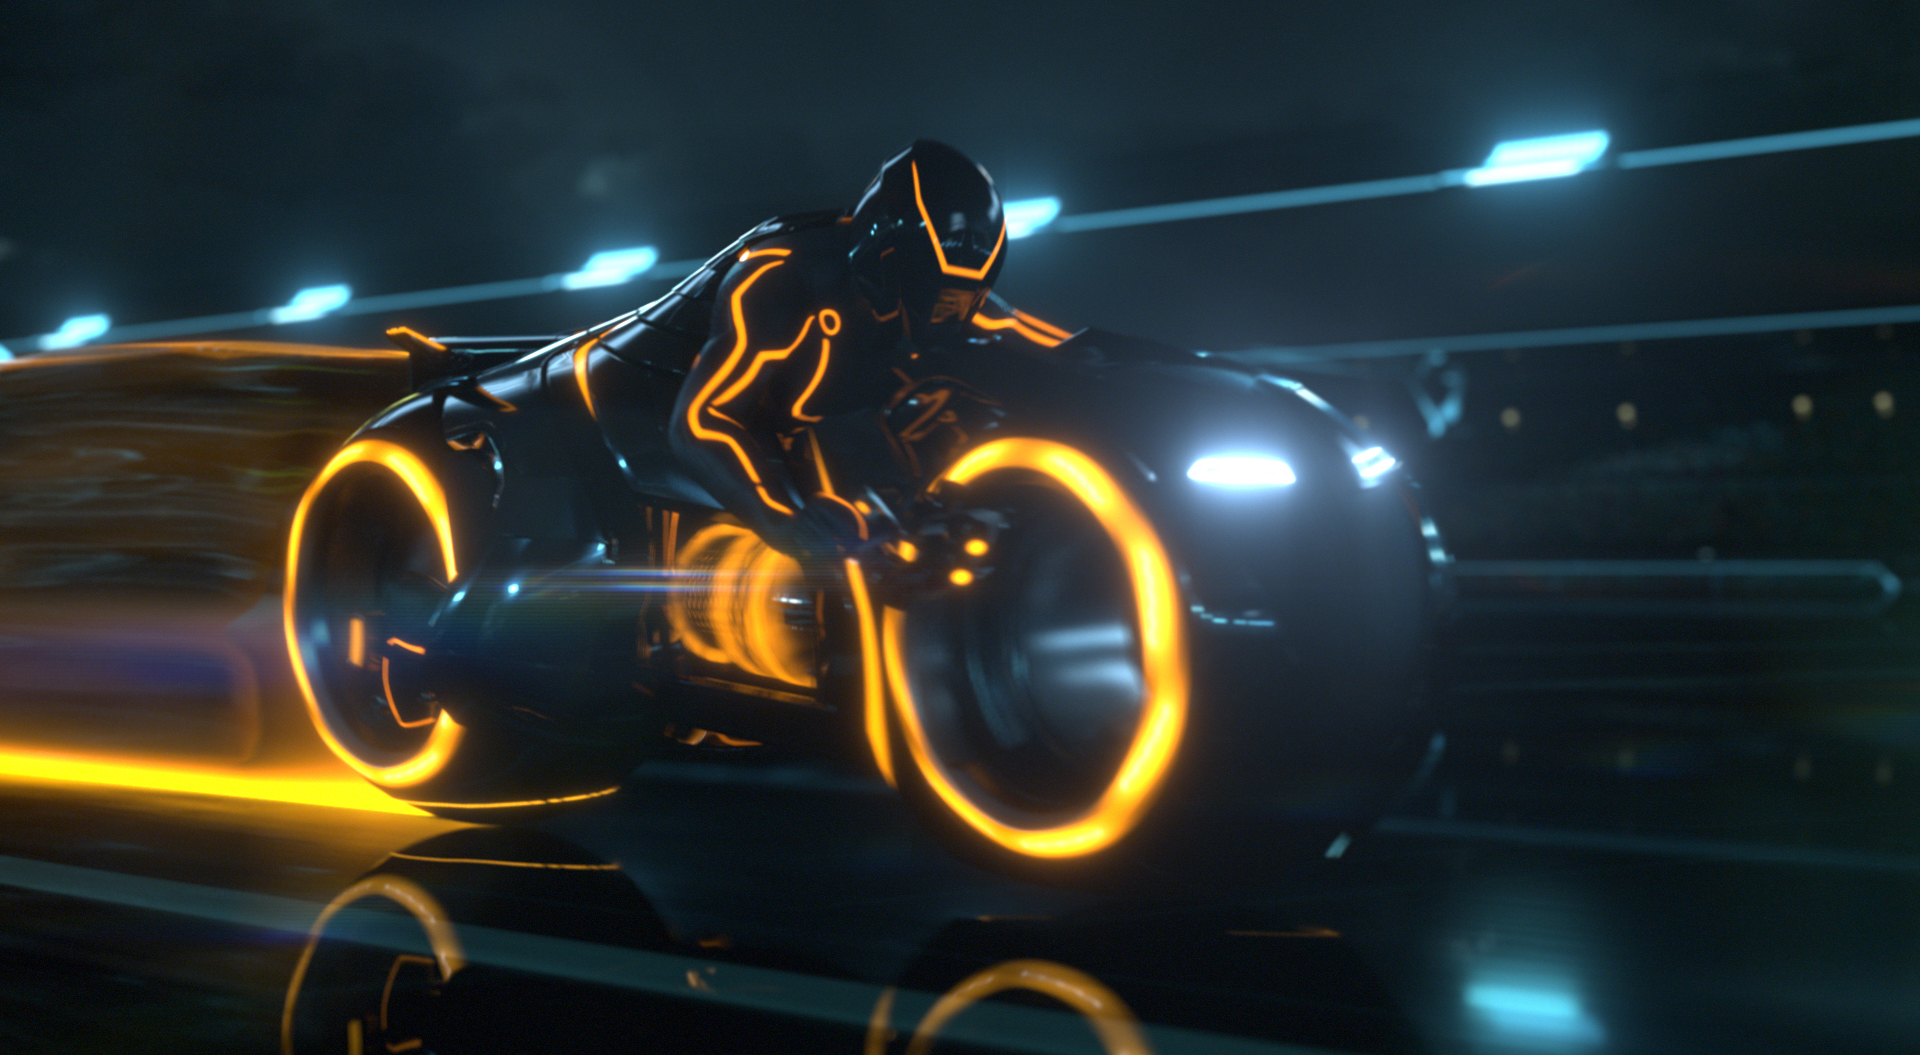
\includegraphics[width=1\textwidth]{figures/Tron-Legacy_Bike.jpg}\\ Tron Licht-Motorräder Computerspiel\\
        \vspace{1cm}
        Bedienungsanleitung \\
        \vspace{0.5cm}
        \small{}ZHAW  School of Engineering
        \vspace{1.cm}
    }
    \author{
        Akca, Deniz\\
        \small{akcaden1@students.zhaw.ch}
        \and
        Holenstein, Christian\\
        \small{holenchr@students.zhaw.ch}
        \and
        Huber, Patrick\\
        \small{huberpa4@students.zhaw.ch}
        \and
        Iten, Mike\\
        \small{itenmik1@students.zhaw.ch}
        \vspace{1.5cm}
    }
   \date{\today}

    \maketitle

    \newpage

    \tableofcontents
	\listoffigures
    \newpage

    \section{Tron Licht-Motorräder Computerspiel}
    Das Tron Licht-Motorräder Computerspiel ist ein netzwerkfähiges \quotes{Remake} des 1982 veröffentlichten Tron Spiels, bzw.  der \quotes{Lichtrenner }-Spielvariante dieses Spieles.

    \section{Beschreibung des Spiels}
    Ein Spieler sieht aus der Draufsicht ein rechteckiges und leeres Spielfeld mit orthogonalen Rasterlinien, das sogenannte \quotes{Grid}. Auf diesem Spielfeld starten mehrere Licht-Motorräder. Der Spieler steuert eines dieser Licht-Motorräder. Jedes Licht-Motorrad zieht während der Fahrt eine Linie (Lichtmauer) nach sich, welche bestehen bleibt. Fährt ein Spieler in eine dieser Lichtmauern, scheidet er aus. Ebenfalls scheidet ein Spieler aus, wenn er in den Spielfeldrand fährt. Gewinner ist schlussendlich, wer im Spiel bleibt, bis alle anderen Spieler ausgeschieden sind.

    \begin{figure}[H]
        \centering
        \makebox[\textwidth][c]{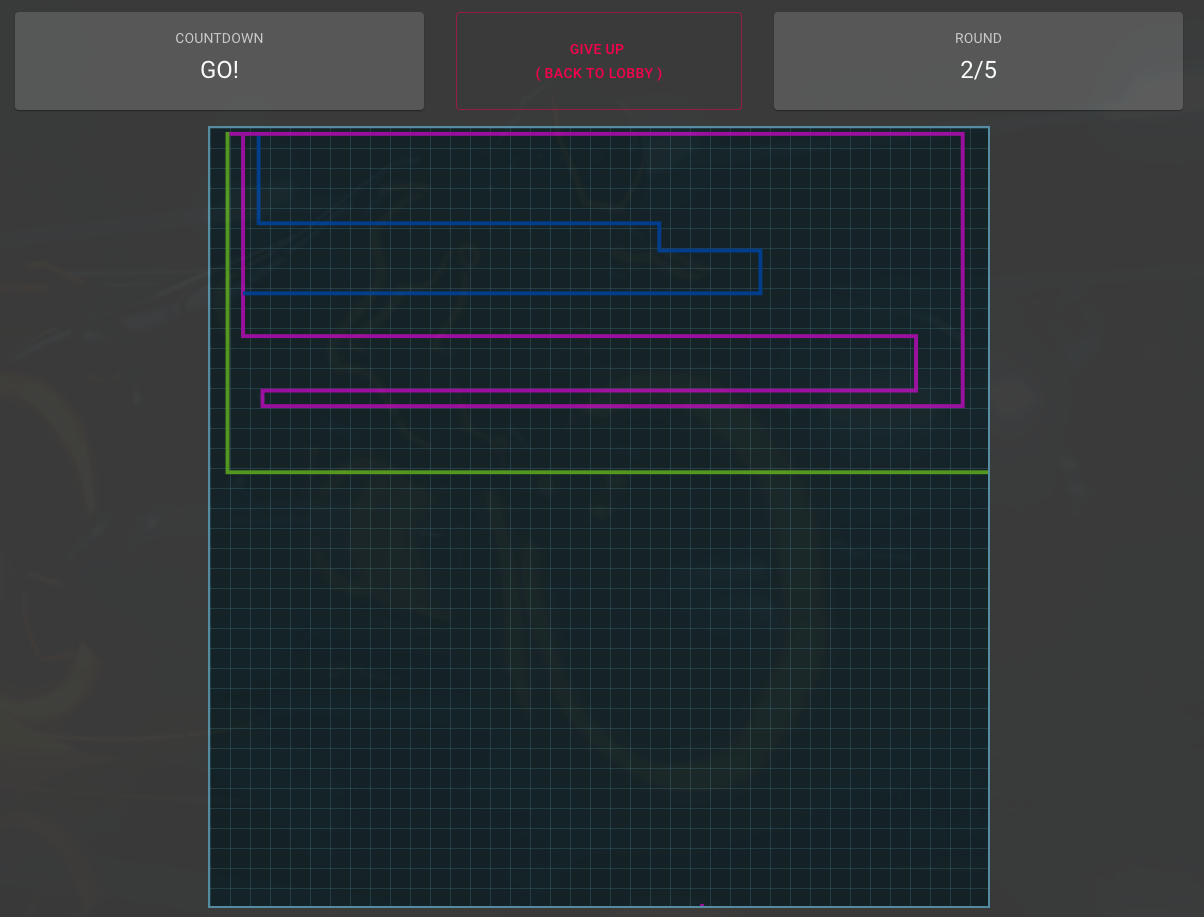
\includegraphics[width=0.95\textwidth]{figures/TheGrid.png}}
        \caption{Tron Licht-Motorräder Computerspiel - \quotes{Grid} Draufsicht}
        \label{fig:TheGrid}
    \end{figure}

   \noindent In \autoref{fig:TheGrid} gut zu erkennen; Das hellblaue Raster ist das Spielfeld und die Linien mit den unterschiedlichen Farben sind die jeweiligen Spieler. Insgesamt sind drei Spieler zu sehen.

    \section{Spielablauf}
    Ein Spiel besteht immer aus einer Lobby und dem Spiel selbst. Die Lobby ist ein Warteraum wo auf andere Spieler gewartet werden kann. Für ein  \quotes{optimales} Spiel, sollten mind. 2 Spieler der Lobby beitreten. Sobald dann alle Spieler bereit sind, kann der Lobbyersteller das Spiel starten.

    \subsection{Public Games}
    \label{ssec:PublicGames}
    Unter \textbf{Public Games} sind alle laufenden Spiele aufgelistet, die von anderen Spielern mit der Sichtbarkeit \quotes{public} erstellt wurden. Wer möchte kann diesen beitreten, falls noch freie Spielerplätze vorhanden sind. \newline
    Im folgenden wird erklärt wie man einem \textbf{Public Game} beitreten kann: \newline
    \newline
    Der User kann über den Button 
\includegraphics{figures/1.png} - wie in \autoref{fig:Spiel_Beitreten} ersichtlich - einem bereits laufenden \textbf{Public Game} bzw. dessen Lobby beitreten.

    \begin{figure}[H]
    	\centering
    	\makebox[\textwidth][c]{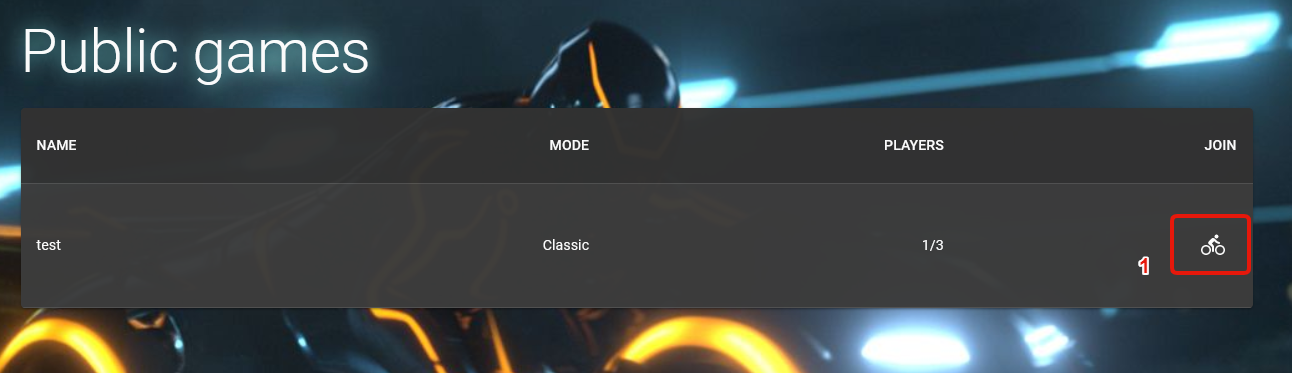
\includegraphics[width=0.95\textwidth]{figures/Spiel_beitreten.png}}
    	\caption{\textbf{Public Game} beitreten}
    	\label{fig:Spiel_Beitreten}
    \end{figure}

    \subsection{Create Game}
    Unter \textbf{Create Game} kann ein neues Spiel erstellt werden. \newline
    \newline
    In \autoref {fig:Spiel_Erstellen} ist ersichtlich, wie ein User sein eigenes Spiel erstellen kann.

	\begin{figure}[H]
		\centering
		\makebox[\textwidth][c]{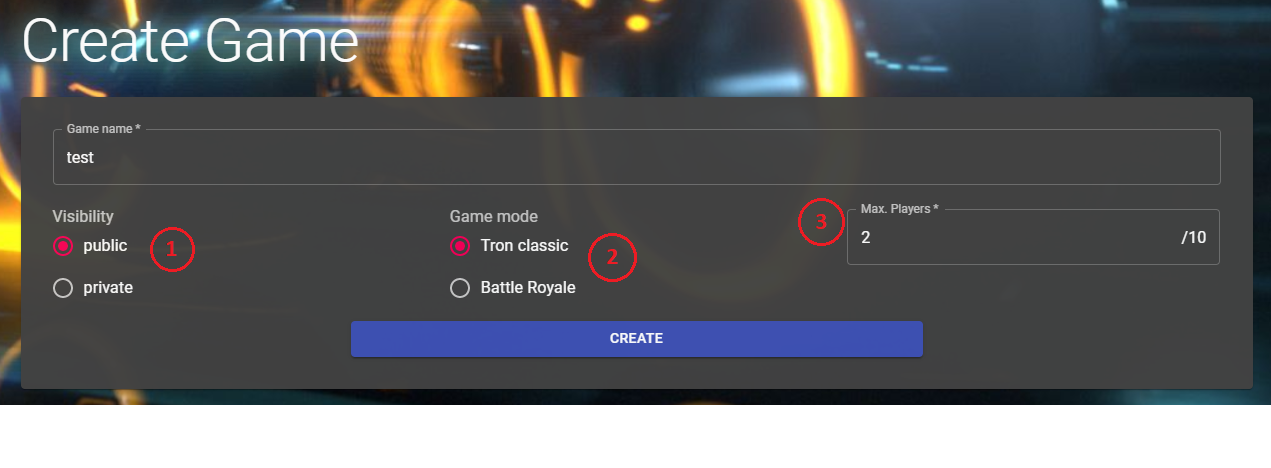
\includegraphics[width=0.95\textwidth]{figures/Spiel_erstellen.png}}
		\caption{Spiel erstellen}
		\label{fig:Spiel_Erstellen}
	\end{figure}

    \noindent 
\includegraphics{figures/1.png} Wird die Sichtbarkeit \quotes{public} ausgewählt, wird das Spiel unter \nameref{ssec:PublicGames} augelistet. \newline
    \newline
    \noindent 
\includegraphics{figures/2.png} \quotes{Tron classic} ist der Standard-Spielemodus, welcher ein klassisches Spiel startet. Diesem können maximal 10 Spieler beitreten. \newline
    Dem \quotes{Battle Royale} Spielemodus können maximal 100 Spieler beitreten.\newline
    \newline
    \noindent 
\includegraphics{figures/3.png} Hier kann die gewünschte maximale Spieleranzahl eingegeben werden. Sobald das Limit erreicht ist, können keine weiteren Spieler mehr beitreten.

    \subsection{Lobby}

    Sobald eine Spiel erstellt wurde, öffnet sich die dazugehörende Lobby. Folgender Ausschnitt ist nun ersichtlich, siehe \autoref{fig:Lobby}:
    \begin{figure}[H]
    	\centering
    	\makebox[\textwidth][c]{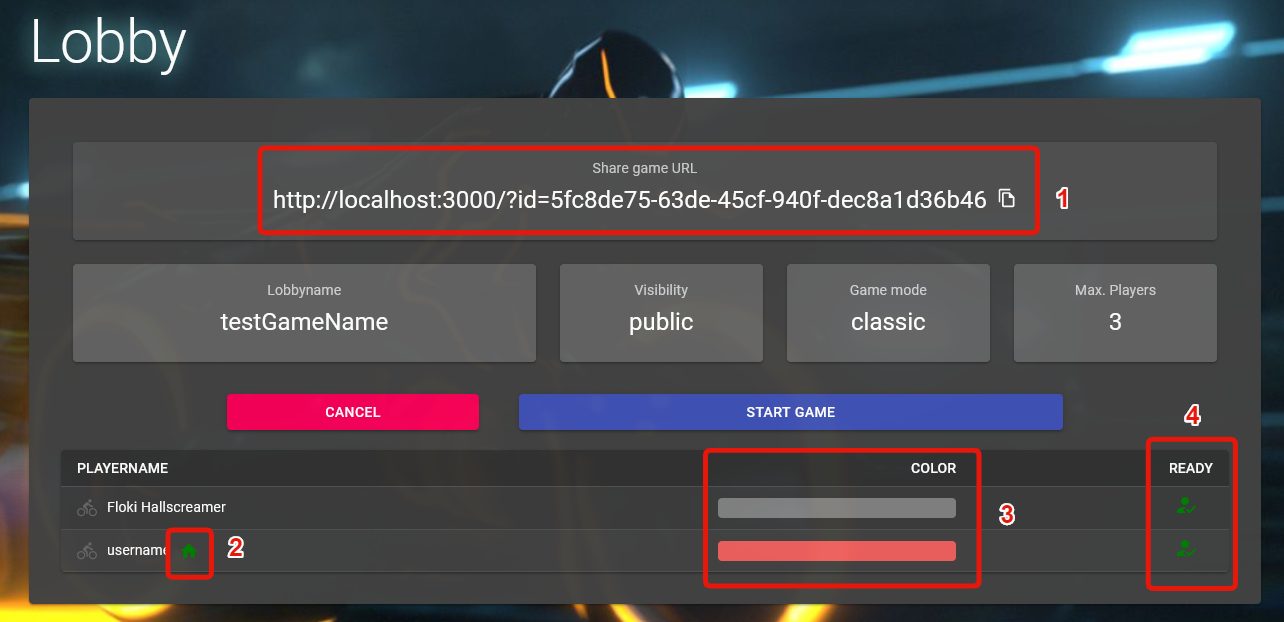
\includegraphics[width=0.95\textwidth]{figures/Lobby.png}}
    	\caption{Lobby}
    	\label{fig:Lobby}
    \end{figure}


    \noindent 
\includegraphics{figures/1.png} Unter \textbf{Share game URL} kann der Link zu diesem Spiel kopiert und an Freunde o. andere potenzielle Mitspieler versendet werden. Falls Mitspieler der Lobby beitreten möchten, können diese den Link in ihrem Browserfenster in die Adresszeile kopieren und - nach einer Bestätigung - der Lobby beitreten.\newline
    \newline
    \noindent 
\includegraphics{figures/2.png} Das grüne Haus signalisiert welcher Spieler der Ersteller der Lobby (Host) ist und somit das Spiel starten kann.\newline
    \newline
    \noindent 
\includegraphics{figures/3.png} Die gewünschte Farbe (für die Lichtmauer und zur Erkennung im Spiel) kann hier für den eigenen Spieler angepasst werden.\newline
    \newline
    \noindent 
\includegraphics{figures/4.png} Sobald alle Spieler ihren Status auf \textbf{ready} geändert haben, kann der Ersteller der Lobby das Spiel starten kann. Solange andere Mitspieler nicht \textbf{ready} sind, ist der \textbf{START GAME} Button deaktiviert.

    \subsection{Spielen}

    Durch klicken des Lobbyerstellers auf den \textbf{START GAME} Button, wird das Spiel gestartet und es erscheint ein Spielfeld. Oberhalb des Spielfeldes befindet sich ein Countdown, welcher mit dem runterzählen beginnt.

    \begin{figure}[H]
        \centering
        \makebox[\textwidth][c]{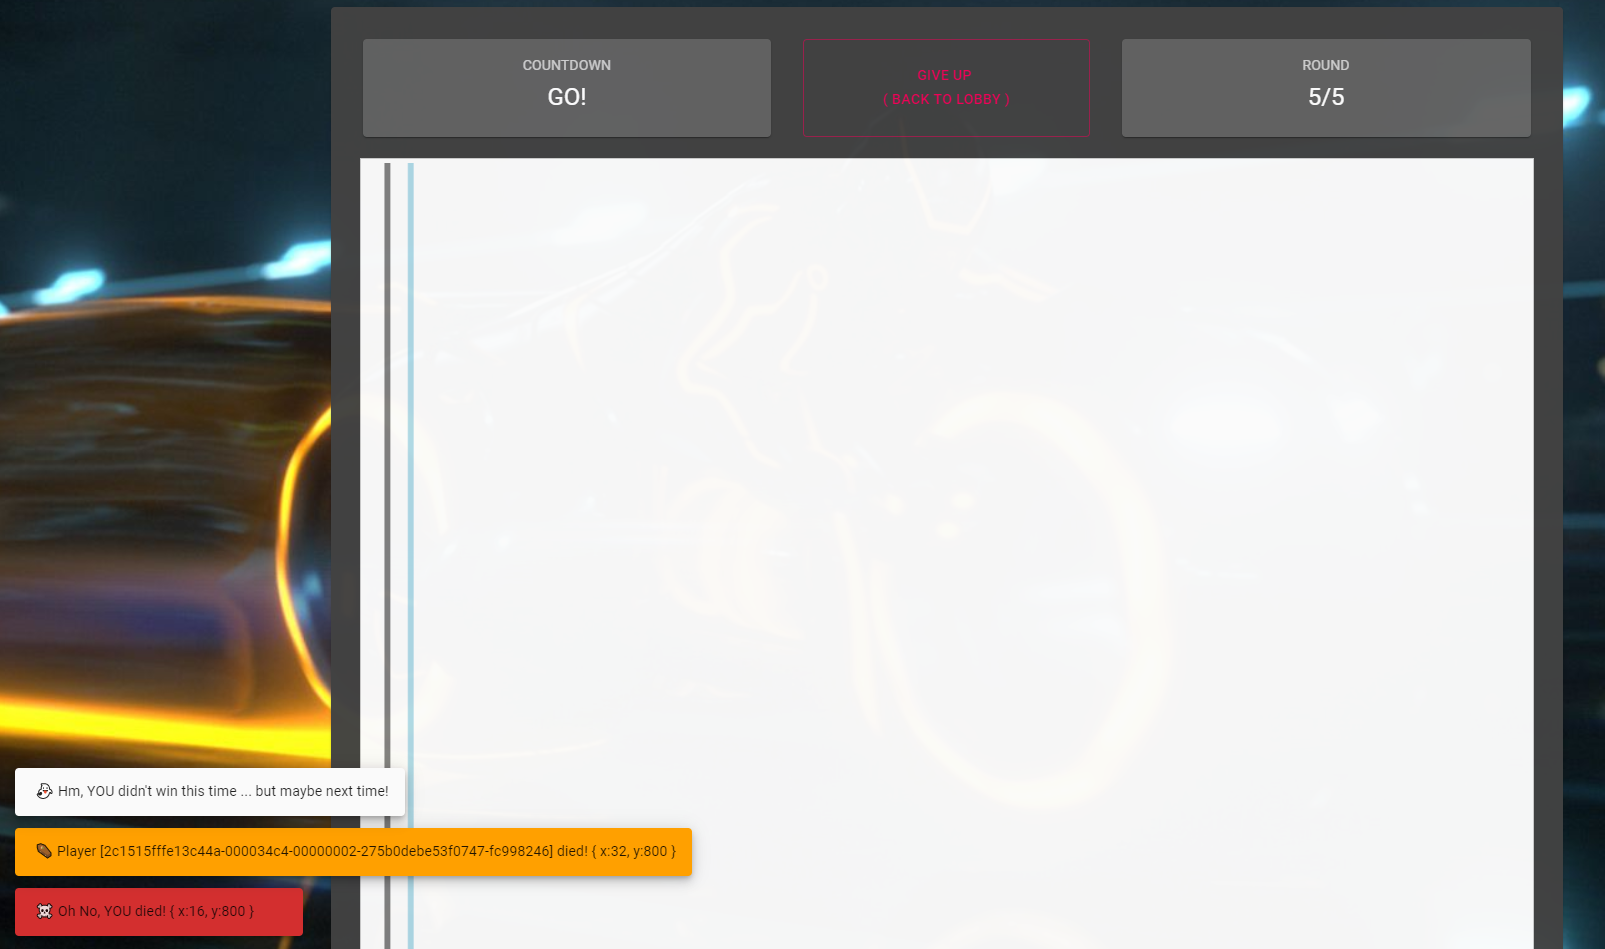
\includegraphics[width=0.95\textwidth]{figures/Spielfeld.png}}
        \caption{Spielfeld mit Countdown- und Rundenanzeige}
        \label{fig:Spielfeld}
    \end{figure}

    \noindent Mit den Pfeiltasten auf der Tastatur kann das Motorrad in die jeweilig gedrückte Richtung navigiert werden.
    In die eigene Lichtmauer oder die der Mitspieler, sollte nicht hineingefahren werden, ebenfalls nicht in den Spielfeldrand. \newline
    \newline
    Während des Spiels können Meldungen über das ausscheiden andere Mitspieler erscheinen, sowie eine Meldung für das eigene ausscheiden. \newline
    \newline
    Schlussendlich ist das Ziel, der letzte Spieler auf dem Spielfeld zu sein. Nach 5 Runden ist ein Spiel vorbei. Nach jeder Runde erscheint eine Nachricht, ob man gewonnen oder verloren hat.

     \section{Anmeldung (optional)}
    Dem User stehen zwei Möglichkeiten zu Verfügung:
    \begin{enumerate}
        \item Gastkonto: Beim erstmaligen Betreten wird automatisch ein Benutzername generiert 
\includegraphics{figures/1.png} (\autoref{fig:Anmeldung}) und der User kann direkt einem Spiel beitreten oder ein Spiel erstellen. Es ist kein Login bzw. Konto nötig.
        \item Registrierung/Login:
        \begin{itemize}
            \item  Falls der User sich registrieren möchte um Punkte für die Statistik zu sammeln, so hat er unter Punkt 
\includegraphics{figures/2.png} (\autoref{fig:Anmeldung}) die Möglichkeit dazu.
            \item Sollte bereits ein Konto vorhanden sein, dann ist der Login unter Punkt 
\includegraphics{figures/3.png} vorzufinden.
        \end{itemize}
    \end{enumerate}

    \begin{figure}[H]
    	\centering
    	\makebox[\textwidth][c]{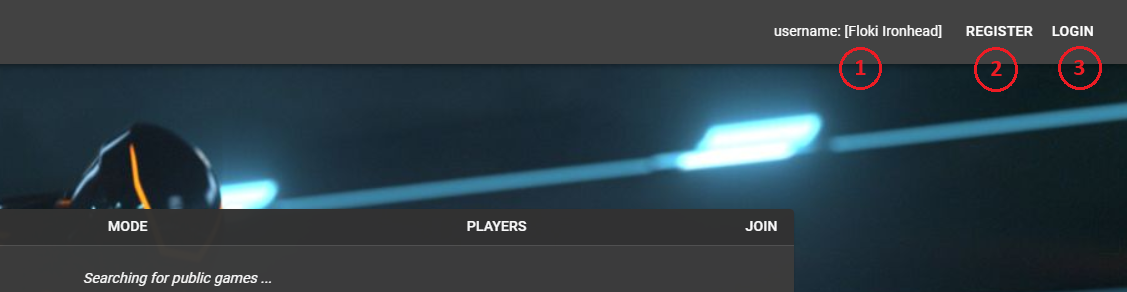
\includegraphics[width=0.95\textwidth]{figures/Anmeldung.png}}
    	\caption{Anmeldung}
    	\label{fig:Anmeldung}
    \end{figure}

    \noindent Nach erfolgreicher Anmeldung, kann der User durch Klick auf das Profilicon unter Punkt 
\includegraphics{figures/1.png} in \autoref{fig:MyAccount} seine Kontoinformationen einsehen/ändern. Ebenfalls kann der User sich dort abmelden.
    % TODO: Bild von dropdown menu?

    \begin{figure}[H]
    	\centering
    	\makebox[\textwidth][c]{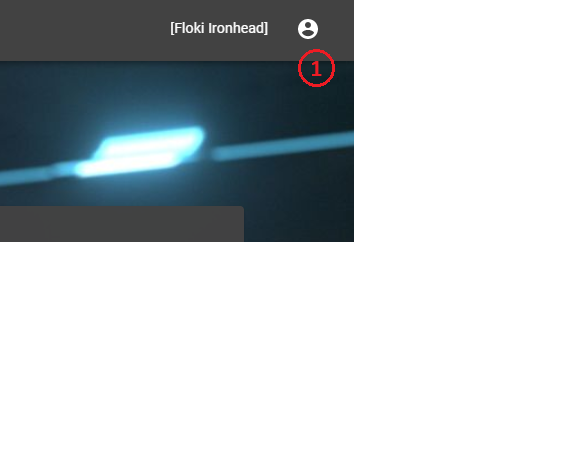
\includegraphics[width=0.95\textwidth]{figures/MyAccount.png}}
    	\caption{Angemeldeter Zustand - Profilicon}
    	\label{fig:MyAccount}
    \end{figure}


\end{document}